\begin{appendices}
	\crefalias{chapter}{appcha}
	\crefalias{section}{appsec}
	\renewcommand{\thesection}{\Alph{chapter}\arabic{section}}

	\chapter{Additional results for \cref{cha:obesity_genetic_signatures_and_cancer}}
	\label{app:a}

	\section{Comparison of the Creighton \textit{et al.} obesity metagene in standardised or non-standardised CR data}
	\label{sec:metagenes_created_from_raw_data_vs_standardised_data}

	\begin{figure}[htpb]
		\centering
		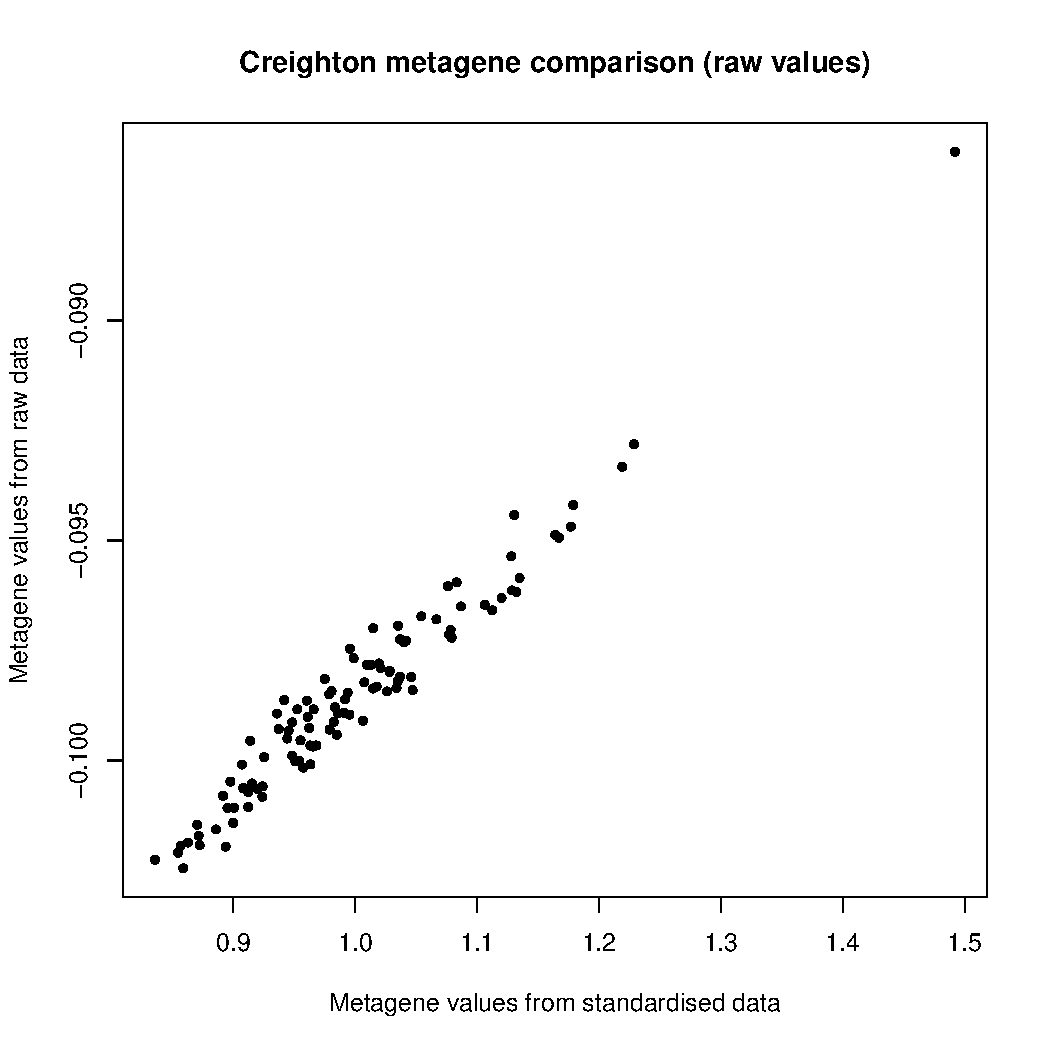
\includegraphics[width=0.45\linewidth,page=1]{appendix/check_raw_vs_std_mg}
		\hfill
		\includegraphics[width=0.45\linewidth,page=2]{appendix/check_raw_vs_std_mg}
		\caption{Scatter plots showing the raw and ranked Creighton \textit{et al.} obesity metagene values generated from standardised or non-standardised CR data set. }
		\label{fig:appendix/check_raw_vs_std}
	\end{figure}

	\section{Comparison of the Creighton \textit{et al.} obesity metagene in standardised or non-standardised \gls{icgc} data}
	\label{sec:comp_cr_raw_std_icgc}

	\begin{figure}[h]
		\centering
		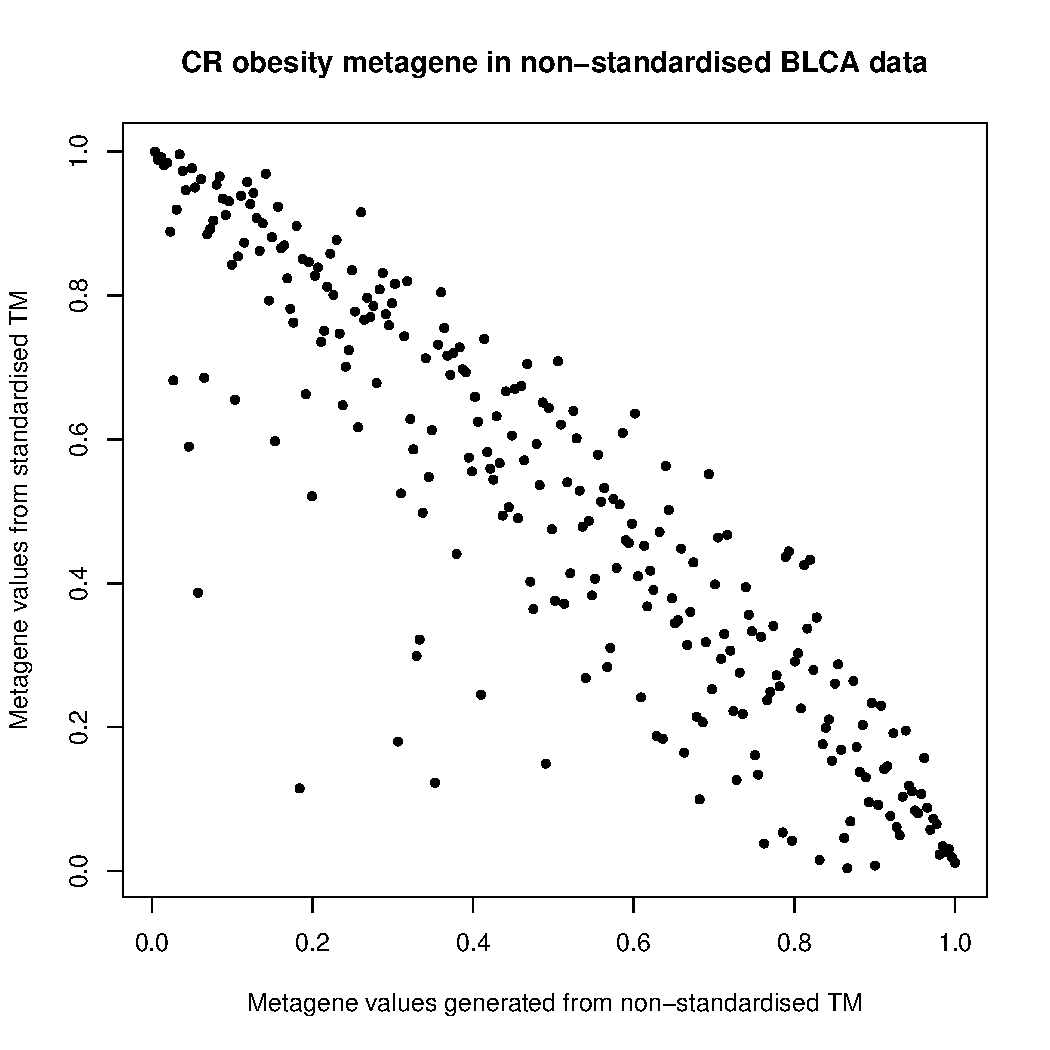
\includegraphics[width=0.45\linewidth,page=1]{appendix/crtcga_raw_vs_std}
		\hfill
		\includegraphics[width=0.45\linewidth,page=2]{appendix/crtcga_raw_vs_std}\\
		\includegraphics[width=0.45\linewidth,page=5]{appendix/crtcga_raw_vs_std}
		\hfill
		\includegraphics[width=0.45\linewidth,page=6]{appendix/crtcga_raw_vs_std}\\
		\caption{Scatter plots comparing the Creighton \textit{et al.} obesity metagene generated from transformation matrix (from standardised or non-standardised CR data) in non-standardised (left) and standardised (right) \gls{icgc} data.}
		\label{fig:appendix/check_raw_vs_std}
	\end{figure}

	\begin{figure}[htpb]
		\ContinuedFloat
		\captionsetup{list=off,format=cont}
		\centering
		\includegraphics[width=0.45\linewidth,page=9]{appendix/crtcga_raw_vs_std}
		\hfill
		\includegraphics[width=0.45\linewidth,page=10]{appendix/crtcga_raw_vs_std}\\
		\includegraphics[width=0.45\linewidth,page=13]{appendix/crtcga_raw_vs_std}
		\hfill
		\includegraphics[width=0.45\linewidth,page=14]{appendix/crtcga_raw_vs_std}\\
		\includegraphics[width=0.45\linewidth,page=17]{appendix/crtcga_raw_vs_std}
		\hfill
		\includegraphics[width=0.45\linewidth,page=18]{appendix/crtcga_raw_vs_std}\\
		\caption{Figure continued}
	\end{figure}

	\begin{figure}[htpb]
		\ContinuedFloat
		\captionsetup{list=off,format=cont}
		\centering
		\includegraphics[width=0.45\linewidth,page=21]{appendix/crtcga_raw_vs_std}
		\hfill
		\includegraphics[width=0.45\linewidth,page=22]{appendix/crtcga_raw_vs_std}\\
		\includegraphics[width=0.45\linewidth,page=25]{appendix/crtcga_raw_vs_std}
		\hfill
		\includegraphics[width=0.45\linewidth,page=26]{appendix/crtcga_raw_vs_std}\\
		\includegraphics[width=0.45\linewidth,page=29]{appendix/crtcga_raw_vs_std}
		\hfill
		\includegraphics[width=0.45\linewidth,page=30]{appendix/crtcga_raw_vs_std}\\
		\caption{Figure continued}
	\end{figure}

	\noindent
	As shown in \cref{fig:appendix/check_raw_vs_std}, the Creighton \textit{et al.} obesity metagene values generated from the transformation matrices (from standardised or non-standardised CR data) were more consistent (or less variable) in the standardised \gls{icgc} data, compared with the non-standardised data.
	Results from \cref{fig:appendix/check_raw_vs_std_tm} suggested that there was no obvious difference in the quality of the metagenes generated from standardised or non-standardised TM.

	\begin{figure}[h]
		\centering
		\includegraphics[width=0.45\linewidth,page=3]{appendix/crtcga_raw_vs_std}
		\hfill
		\includegraphics[width=0.45\linewidth,page=4]{appendix/crtcga_raw_vs_std}\\
		\includegraphics[width=0.45\linewidth,page=7]{appendix/crtcga_raw_vs_std}
		\hfill
		\includegraphics[width=0.45\linewidth,page=8]{appendix/crtcga_raw_vs_std}\\
		\caption{Scatter plots comparing the Creighton \textit{et al.} obesity metagene generated from transformation matrix from non-standardisedright (left) or standardised (right) CR data in non-standardised  and standardised  \gls{icgc} data.}
		\label{fig:appendix/check_raw_vs_std_tm}
	\end{figure}

	\begin{figure}[htpb]
		\ContinuedFloat
		\captionsetup{list=off,format=cont}
		\centering
		\includegraphics[width=0.45\linewidth,page=11]{appendix/crtcga_raw_vs_std}
		\hfill
		\includegraphics[width=0.45\linewidth,page=12]{appendix/crtcga_raw_vs_std}\\
		\includegraphics[width=0.45\linewidth,page=15]{appendix/crtcga_raw_vs_std}
		\hfill
		\includegraphics[width=0.45\linewidth,page=16]{appendix/crtcga_raw_vs_std}\\
		\includegraphics[width=0.45\linewidth,page=19]{appendix/crtcga_raw_vs_std}
		\hfill
		\includegraphics[width=0.45\linewidth,page=20]{appendix/crtcga_raw_vs_std}\\
		\caption{Figure continued}
	\end{figure}

	\begin{figure}[htpb]
		\ContinuedFloat
		\captionsetup{list=off,format=cont}
		\centering
		\includegraphics[width=0.45\linewidth,page=23]{appendix/crtcga_raw_vs_std}
		\hfill
		\includegraphics[width=0.45\linewidth,page=24]{appendix/crtcga_raw_vs_std}\\
		\includegraphics[width=0.45\linewidth,page=27]{appendix/crtcga_raw_vs_std}
		\hfill
		\includegraphics[width=0.45\linewidth,page=28]{appendix/crtcga_raw_vs_std}\\
		\includegraphics[width=0.45\linewidth,page=31]{appendix/crtcga_raw_vs_std}
		\hfill
		\includegraphics[width=0.45\linewidth,page=32]{appendix/crtcga_raw_vs_std}\\
		\caption{Figure continued}
	\end{figure}

	\section{Remainder of the results of Creighton \textit{et al.} obesity metagene in \gls{icgc} cancer data sets}
	\label{sec:rest_of_the_cr_icgc_cancer_heatmap_results}

	\begin{figure}[htp!]
		\centering
		\includegraphics[width=0.45\linewidth,page=8]{appendix/crtcga_std}\\
		\vspace{1em}
		\includegraphics[width=0.45\linewidth,page=13]{appendix/crtcga_std}
		\hfill
		\includegraphics[width=0.45\linewidth,page=18]{appendix/crtcga_std}\\
		\caption{Heatmaps showing the association of obesity metagene from the \citet{Creighton2012} study with sample gene expression from the other \gls{icgc} data sets.
	Level of expression is represented in the top right histogram, where low and high gene expression were colour-coded with blue and red, respectively.
	Each row of the heatmap represents a gene from the obesity associated genetic signature, and each column of the heatmap represents a sample from the \gls{icgc} data.
	The obesity associated metagene scores of the samples are shown in a separate row at top of the heatmap, and the tree diagram of the heirarchical clustering of the genes is shown to the left of the heatmap. }
		\label{fig:appendix/cr_icgc_heatmap}
	\end{figure}

	\begin{figure}[htpb]
		\ContinuedFloat
		\captionsetup{list=off,format=cont}
		\centering
		\includegraphics[width=0.45\linewidth,page=23]{appendix/crtcga_std}
		\hfill
		\includegraphics[width=0.45\linewidth,page=28]{appendix/crtcga_std}\\
		\vspace{1em}
		\includegraphics[width=0.45\linewidth,page=33]{appendix/crtcga_std}
		\hfill
		\includegraphics[width=0.45\linewidth,page=38]{appendix/crtcga_std}\\
		\vspace{1em}
		\caption{figure}
	\end{figure}

	\noindent
	As shown in \cref{fig:appendix/cr_icgc_heatmap}, the obesity metagene from the Creighton \textit{et al.} study was reflective of the sample gene expression levels of the obesity associated genetic signature in all of the other \gls{icgc} cancer data sets.
	However, none of the \gls{icgc} cancer data sets (other than the \gls{blca} data set; \cref{fig:crmetaicgc} in \cref{sec:creighton_obesity_metagene}) showed any significant association of the sample \gls{bmi} or \gls{bmi} status with the Creighton \textit{et al.} obesity metagene (\cref{fig:appendix/cr_icgc_box_scatter}).

	\begin{figure}[htpb]
		\centering
		\includegraphics[page=9,width=0.45\linewidth]{appendix/crtcga_std}
		\hfill
		\includegraphics[page=10,width=0.45\linewidth]{appendix/crtcga_std}\\
		\includegraphics[page=14,width=0.45\linewidth]{appendix/crtcga_std}
		\hfill
		\includegraphics[page=15,width=0.45\linewidth]{appendix/crtcga_std}\\
		\caption{Box plots and scatter plots showing the association of obesity metagene from the \citet{Creighton2012} study with the sample \gls{bmi} status  and \gls{bmi} from the other \gls{icgc} data sets, respectively.
	In the box plot, the p-values above the groups represent the statistical significance of the association of the metagene with the overweight or obese group compared with the normal weight group.
	The \gls{anova} p-value shows the statistical significance of the association of the metagene with the sample \gls{bmi} groups.
	In the scatter plot, $R^2$- and p-values describe the adjusted coefficient of determination of the regression line and the statistical significance of the linear model used to draw the regression line, respectively.}
		\label{fig:appendix/cr_icgc_box_scatter}
	\end{figure}

	\begin{figure}[htpb]
		\ContinuedFloat
		\captionsetup{list=off,format=cont}
		\centering
		\includegraphics[page=19,width=0.45\linewidth]{appendix/crtcga_std}
		\hfill
		\includegraphics[page=20,width=0.45\linewidth]{appendix/crtcga_std}\\
		\includegraphics[page=24,width=0.45\linewidth]{appendix/crtcga_std}
		\hfill
		\includegraphics[page=25,width=0.45\linewidth]{appendix/crtcga_std}\\
		\includegraphics[page=29,width=0.45\linewidth]{appendix/crtcga_std}
		\hfill
		\includegraphics[page=30,width=0.45\linewidth]{appendix/crtcga_std}\\
		\caption{Name}
	\end{figure}

	\begin{figure}[htpb]
		\ContinuedFloat
		\captionsetup{list=off,format=cont}
		\centering
		\includegraphics[page=34,width=0.45\linewidth]{appendix/crtcga_std}
		\hfill
		\includegraphics[page=35,width=0.45\linewidth]{appendix/crtcga_std}\\
		\includegraphics[page=39,width=0.45\linewidth]{appendix/crtcga_std}
		\hfill
		\includegraphics[page=40,width=0.45\linewidth]{appendix/crtcga_std}\\
		\caption{Name}
	\end{figure}

	\section{Comparison of the FM obesity metagene in standardised or non-standardised FM data}
	\label{sec:fm_metagene_raw_vs_std}

	\noindent
	\cref{fig:appendix/fm_meta_check} suggested that the FM obesity associated genetic signature was noisy, unlike the Creighton \textit{et al.} signature (\cref{fig:appendix/check_raw_vs_std}).
	The heatmaps in \cref{fig:appendix/fm_meta_heat} showed further evidence of the FM genetic signature being noisy and of poor quality, as the FM metagene did not reflect the sample gene expression patterns as well as the obesity associated genetic signature from the Creighton \textit{et al.} study.

	\begin{figure}[htpb]
		\centering
		\includegraphics[page=1,width=0.45\linewidth]{appendix/fm_meta_check}
		\hfill
		\includegraphics[page=2,width=0.45\linewidth]{appendix/fm_meta_check}\\
		\caption{Scatter plots showing the raw and ranked FM obesity metagene values generated from standardised or non-standardised FM data set. }
		\label{fig:appendix/fm_meta_check}
	\end{figure}
	
	\begin{figure}[htpb]
		\centering
		\includegraphics[page=5,width=0.45\linewidth]{appendix/fm_meta_check}
		\hfill
		\includegraphics[page=8,width=0.45\linewidth]{appendix/fm_meta_check}\\
		\caption{Heatmaps showing the association of obesity metagene from the Fuentes-Mattei \textit{et al.} study with sample gene expression from the FM data set.
		Scales are as described in previous figures.}
		\label{fig:appendix/fm_meta_heat}
	\end{figure}

	\section{Remainder of the results of FM obesity metagene in \gls{icgc} cancer data sets}
	\label{sec:rest_of_the_fm_icgc_cancer_heatmap_results}

	\noindent
	The FM obesity metagene from was reflective of the sample gene expression levels of the obesity associated genetic signature in all of the other \gls{icgc} cancer data sets (\cref{fig:appendix/fm_icgc_heatmap}).
	However, none of the \gls{icgc} cancer data sets (other than the \gls{blca} data set; \cref{fig:fmmetaicgc} in \cref{sec:fm_obesity_metagene}) showed any significant association of the sample \gls{bmi} or \gls{bmi} status with the FM obesity metagene (\cref{fig:appendix/fm_icgc_box_scatter}).

	\begin{figure}[htp!]
		\centering
		\includegraphics[width=0.45\linewidth,page=8]{appendix/fm_meta_ICGC}
		\vspace{1em}
		\includegraphics[width=0.45\linewidth,page=13]{appendix/fm_meta_ICGC}\\
		\hfill
		\caption{Heatmaps showing the association of obesity metagene from the \citet{Creighton2012} study with sample gene expression from the other \gls{icgc} data sets.
	Scales are as described in previous figures.}
		\label{fig:appendix/fm_icgc_heatmap}
	\end{figure}

	\begin{figure}[htpb]
		\ContinuedFloat
		\captionsetup{list=off,format=cont}
		\centering
		\includegraphics[width=0.45\linewidth,page=18]{appendix/fm_meta_ICGC}\\
		\vspace{1em}
		\includegraphics[width=0.45\linewidth,page=23]{appendix/fm_meta_ICGC}
		\hfill
		\includegraphics[width=0.45\linewidth,page=28]{appendix/fm_meta_ICGC}\\
		\vspace{1em}
		\includegraphics[width=0.45\linewidth,page=33]{appendix/fm_meta_ICGC}
		\hfill
		\includegraphics[width=0.45\linewidth,page=38]{appendix/fm_meta_ICGC}\\
		\vspace{1em}
		\caption{figure}
	\end{figure}

	\begin{figure}[htpb]
		\centering
		\includegraphics[page=9,width=0.45\linewidth]{appendix/fm_meta_icgc}
		\hfill
		\includegraphics[page=10,width=0.45\linewidth]{appendix/fm_meta_icgc}\\
		\includegraphics[page=14,width=0.45\linewidth]{appendix/fm_meta_icgc}
		\hfill
		\includegraphics[page=15,width=0.45\linewidth]{appendix/fm_meta_icgc}\\
		\caption{Box plots and scatter plots showing the association of obesity metagene from the \citet{Creighton2012} study with the sample \gls{bmi} status  and \gls{bmi} from the other \gls{icgc} data sets, respectively.
	P-values and $R^2$-value are as described in previous figures.}
		\label{fig:appendix/fm_icgc_box_scatter}
	\end{figure}

	\begin{figure}[htpb]
		\ContinuedFloat
		\captionsetup{list=off,format=cont}
		\centering
		\includegraphics[page=19,width=0.45\linewidth]{appendix/fm_meta_icgc}
		\hfill
		\includegraphics[page=20,width=0.45\linewidth]{appendix/fm_meta_icgc}\\
		\includegraphics[page=24,width=0.45\linewidth]{appendix/fm_meta_icgc}
		\hfill
		\includegraphics[page=25,width=0.45\linewidth]{appendix/fm_meta_icgc}\\
		\includegraphics[page=29,width=0.45\linewidth]{appendix/fm_meta_icgc}
		\hfill
		\includegraphics[page=30,width=0.45\linewidth]{appendix/fm_meta_icgc}\\
		\caption{Name}
	\end{figure}

	\begin{figure}[htpb]
		\ContinuedFloat
		\captionsetup{list=off,format=cont}
		\centering
		\includegraphics[page=34,width=0.45\linewidth]{appendix/fm_meta_icgc}
		\hfill
		\includegraphics[page=35,width=0.45\linewidth]{appendix/fm_meta_icgc}\\
		\includegraphics[page=39,width=0.45\linewidth]{appendix/fm_meta_icgc}
		\hfill
		\includegraphics[page=40,width=0.45\linewidth]{appendix/fm_meta_icgc}\\
		\caption{Name}
	\end{figure}

	\section{Creighton DEG metagene direction}
	\label{sec:creighton_deg_metagene_direction}

	To determine the correct direction of each of the novel obesity metagenes obtained from the CR data, heatmaps were created in the CR data.
	Genes that were common to all eight obesity associated genetic signatures were used in the heatmaps to make sure the genes and their expressions were the same in every heatmap.
	The heatmaps from \cref{fig:cr_meta_direction} clearly showed that the Res, ResOl and CaRes obesity metagenes were in the opposite direction compared to the other obesity metagenes, and therefore the three obesity metagenes were flipped in the subsequent analyses.

	\begin{figure}[htpb]
		\centering
		\includegraphics[page=3,width=0.45\linewidth]{appendix/cr_meta_direction_raw}
		\hfill
		\includegraphics[page=6,width=0.45\linewidth]{appendix/cr_meta_direction_raw}\\
		\caption{Heatmaps showing the association of all the novel obesity metagenes from the CR data set with the sample gene expression in CR the data set.
		Genes that were common to all of the novel obesity associated genetic signatures were used in the heatmap.
		Scales are as described in previous figures.}
		\label{fig:cr_meta_direction}
	\end{figure}

	\begin{figure}[htpb]
		\ContinuedFloat
		\captionsetup{list=off,format=cont}
		\centering
		\includegraphics[page=9,width=0.45\linewidth]{appendix/cr_meta_direction_raw}
		\hfill
		\includegraphics[page=12,width=0.45\linewidth]{appendix/cr_meta_direction_raw}\\
		\vspace{1em}
		\includegraphics[page=15,width=0.45\linewidth]{appendix/cr_meta_direction_raw}
		\hfill
		\includegraphics[page=18,width=0.45\linewidth]{appendix/cr_meta_direction_raw}\\
		\vspace{1em}
		\includegraphics[page=21,width=0.45\linewidth]{appendix/cr_meta_direction_raw}
		\hfill
		\includegraphics[page=24,width=0.45\linewidth]{appendix/cr_meta_direction_raw}\\
		\caption{Name}
	\end{figure}

	\section{Number of gene probes/genes in each of the obesity associated genetic signature}
	\label{app:number_of_gene_probes_genes_in_each_signature}

	Since all of the genes in the obesity associated genetic signatures from the CR data were in terms of the microarray gene probes rather than gene symbols, the gene probes were converted into gene symbols.
	Furthermore, since some gene symbols were not present in the \gls{icgc} data, these genes were omitted from the analyses.
	Therefore, the final number of genes used in the analyses in this project were slightly less than the number of genes originally identified.
	The final number of genes for each of the obesity associated genetic signatures were summarised in \cref{tab:signature_gene_num}.

	\begin{table}[htbp]
		\centering
		\caption{Summary of the number of gene probes and gene symbols for each of the obesity associated genetic signatures identified from the CR data}
		\label{tab:signature_gene_num}
		\begin{tabular}{lcc}
			Obesity associated genetic signature & No. gene probes   & No. gene symbols\\
			\hline
			\rule{0pt}{2.25ex}Or & 799 & 644 \\
			Cr                   & 799 & 678 \\
			Res                  & 799 & 655 \\
			Ca                   & 799 & 657 \\
			CaRes                & 799 & 651 \\
			CrOl                 & 239 & 199 \\
			ResOl                & 168 & 147 \\
			CaOl                 & 148 & 128 \\
			CaResOl              & 92  & 86  \\
			\hline
			\hline
		\end{tabular}
	\end{table}

	\section{Remainder of the results of the other CR obesity metagenes in CR data set}
	\label{sec:rest_of_the_cr_ob_meta_heatmap_results}

	As already mentioned in \cref{sub:_novel_obesity_associated_signatures_and_sample_bmi}, all of the obesity associated geneti signatures derived from the CR data captured the overall gene expressions in the CR data, and significantly correlated with the sample \gls{bmi}/\gls{bmi} status (\cref{fig:appendix/cr_ob_meta_heatmap,fig:appendix/cr_ob_meta_box_scatter}).

	\begin{figure}[htp!]
		\centering
		\includegraphics[width=0.45\linewidth,page=8]{appendix/cr_deg_meta_vs_clin}\\
		\vspace{1em}
		\includegraphics[width=0.45\linewidth,page=13]{appendix/cr_deg_meta_vs_clin}
		\hfill
		\includegraphics[width=0.45\linewidth,page=18]{appendix/cr_deg_meta_vs_clin}\\
		\vspace{1em}
		\includegraphics[width=0.45\linewidth,page=23]{appendix/cr_deg_meta_vs_clin}
		\hfill
		\includegraphics[width=0.45\linewidth,page=28]{appendix/cr_deg_meta_vs_clin}\\
		\caption{Heatmaps showing the association of the other CR obesity metagenes with the sample gene expression from the CR data set.
	Scales are as described in previous figures.}
		\label{fig:appendix/cr_ob_meta_heatmap}
	\end{figure}

	\begin{figure}[htpb]
		\ContinuedFloat
		\captionsetup{list=off,format=cont}
		\centering
		\includegraphics[width=0.45\linewidth,page=33]{appendix/cr_deg_meta_vs_clin}
		\hfill
		\includegraphics[width=0.45\linewidth,page=38]{appendix/cr_deg_meta_vs_clin}\\
		\vspace{1em}
		\caption{figure}
	\end{figure}

	\begin{figure}[htpb]
		\centering
		\includegraphics[page=9,width=0.45\linewidth]{appendix/cr_deg_meta_vs_clin}
		\hfill
		\includegraphics[page=10,width=0.45\linewidth]{appendix/cr_deg_meta_vs_clin}\\
		\caption{Box plots and scatter plots showing the association of the other CR obesity metagenes with the sample \gls{bmi} status  and \gls{bmi} from the CR data set, respectively.
	P-values and $R^2$-value are as described in previous figures.}
		\label{fig:appendix/cr_ob_meta_box_scatter}
	\end{figure}

	\begin{figure}[htpb]
		\ContinuedFloat
		\captionsetup{list=off,format=cont}
		\centering
		\includegraphics[page=14,width=0.45\linewidth]{appendix/cr_deg_meta_vs_clin}
		\hfill
		\includegraphics[page=15,width=0.45\linewidth]{appendix/cr_deg_meta_vs_clin}\\
		\includegraphics[page=19,width=0.45\linewidth]{appendix/cr_deg_meta_vs_clin}
		\hfill
		\includegraphics[page=20,width=0.45\linewidth]{appendix/cr_deg_meta_vs_clin}\\
		\includegraphics[page=24,width=0.45\linewidth]{appendix/cr_deg_meta_vs_clin}
		\hfill
		\includegraphics[page=25,width=0.45\linewidth]{appendix/cr_deg_meta_vs_clin}\\
		\caption{Name}
	\end{figure}

	\begin{figure}[htpb]
		\ContinuedFloat
		\captionsetup{list=off,format=cont}
		\centering
		\includegraphics[page=29,width=0.45\linewidth]{appendix/cr_deg_meta_vs_clin}
		\hfill
		\includegraphics[page=30,width=0.45\linewidth]{appendix/cr_deg_meta_vs_clin}\\
		\includegraphics[page=34,width=0.45\linewidth]{appendix/cr_deg_meta_vs_clin}
		\hfill
		\includegraphics[page=35,width=0.45\linewidth]{appendix/cr_deg_meta_vs_clin}\\
		\includegraphics[page=39,width=0.45\linewidth]{appendix/cr_deg_meta_vs_clin}
		\hfill
		\includegraphics[page=40,width=0.45\linewidth]{appendix/cr_deg_meta_vs_clin}\\
		\caption{Name}
	\end{figure}

	\section{Remainder of the results of the other CR obesity metagenes in \gls{icgc} data sets}
	\label{sec:rest_of_the_cr_ob_meta_heatmap_results_icgc}

	In the \gls{icgc} data sets, \gls{blca} data set was the only \gls{icgc} data set to show any significant association with the sample \gls{bmi} status.
	All of the other \gls{icgc} cancer data sets showed no significant association with the sample \gls{bmi}/\gls{bmi} status, but the metagenes were reflective of the sample gene expressions in all of the cancer types.
	For clarity and convenience, results will be split based on the \gls{icgc} cancer type.

	\subsubsection{\gls{blca}}
	\label{ssub:blca}
	
	\begin{figure}[htp!]
		\centering
		\includegraphics[page=3,width=0.45\linewidth]{appendix/crolgene_ICGC}\\
		\vspace{1em}
		\includegraphics[page=3,width=0.45\linewidth]{appendix/resobsgene_ICGC}
		\hfill
		\includegraphics[page=3,width=0.45\linewidth]{appendix/rescrolgene_ICGC}\\
		\caption{Heatmaps showing the association of the other CR obesity metagenes with the sample gene expression from the \gls{icgc} \gls{blca} data set.
		Scales, p-values and $R^2$-value are as described in previous figures.}
		\label{fig:degmetaicgc_blca}
	\end{figure}

	\begin{figure}[htpb]
		\ContinuedFloat
		\captionsetup{list=off,format=cont}
		\centering
		\includegraphics[page=3,height=0.43\linewidth,width=0.45\linewidth]{appendix/caobsgene_ICGC}
		\hfill
		\includegraphics[page=3,height=0.43\linewidth,width=0.45\linewidth]{appendix/cacrolgene_ICGC}\\
		\includegraphics[page=3,height=0.43\linewidth,width=0.45\linewidth]{appendix/caresobsgene_ICGC}
		\hfill
		\includegraphics[page=3,height=0.43\linewidth,width=0.45\linewidth]{appendix/carescrolgene_ICGC}\\
		\caption{Name}
	\end{figure}

	\begin{figure}[htpb]
		\centering
		\includegraphics[page=4,width=0.45\linewidth]{appendix/crolgene_ICGC}
		\hfill
		\includegraphics[page=5,width=0.45\linewidth]{appendix/crolgene_ICGC}\\
		\caption{Box plots and scatter plots showing the association of the other CR obesity metagenes with the sample \gls{bmi} status  and \gls{bmi} from the \gls{icgc} \gls{blca} data set, respectively.
	P-values and $R^2$-value are as described in previous figures.}
		\label{fig:appendix/cr_ob_meta_box_scatter_blca}
	\end{figure}

	\begin{figure}[htpb]
		\ContinuedFloat
		\captionsetup{list=off,format=cont}
		\centering
		\includegraphics[page=4,width=0.45\linewidth]{appendix/resobsgene_ICGC}
		\hfill
		\includegraphics[page=5,width=0.45\linewidth]{appendix/resobsgene_ICGC}\\
		\includegraphics[page=4,width=0.45\linewidth]{appendix/rescrolgene_ICGC}
		\hfill
		\includegraphics[page=5,width=0.45\linewidth]{appendix/rescrolgene_ICGC}\\
		\includegraphics[page=4,width=0.45\linewidth]{appendix/caobsgene_ICGC}
		\hfill
		\includegraphics[page=5,width=0.45\linewidth]{appendix/caobsgene_ICGC}\\
		\caption{Name}
	\end{figure}

	\begin{figure}[htpb]
		\ContinuedFloat
		\captionsetup{list=off,format=cont}
		\centering
		\includegraphics[page=4,width=0.45\linewidth]{appendix/cacrolgene_ICGC}
		\hfill
		\includegraphics[page=5,width=0.45\linewidth]{appendix/cacrolgene_ICGC}\\
		\includegraphics[page=4,width=0.45\linewidth]{appendix/caresobsgene_ICGC}
		\hfill
		\includegraphics[page=5,width=0.45\linewidth]{appendix/caresobsgene_ICGC}\\
		\includegraphics[page=4,width=0.45\linewidth]{appendix/carescrolgene_ICGC}
		\hfill
		\includegraphics[page=5,width=0.45\linewidth]{appendix/carescrolgene_ICGC}\\
		\caption{Name}
	\end{figure}

	\newpage

	\subsubsection{\gls{cesc}}
	\label{ssub:cesc}
	
	\begin{figure}[htp!]
		\centering
		\includegraphics[page=8,height=0.43\linewidth,width=0.45\linewidth]{appendix/rawobsgene_ICGC}
		\hfill
		\includegraphics[page=8,height=0.43\linewidth,width=0.45\linewidth]{appendix/crolgene_ICGC}\\
		\includegraphics[page=8,height=0.43\linewidth,width=0.45\linewidth]{appendix/resobsgene_ICGC}
		\hfill
		\includegraphics[page=8,height=0.43\linewidth,width=0.45\linewidth]{appendix/rescrolgene_ICGC}\\
		\includegraphics[page=8,height=0.43\linewidth,width=0.45\linewidth]{appendix/caobsgene_ICGC}
		\hfill
		\includegraphics[page=8,height=0.43\linewidth,width=0.45\linewidth]{appendix/cacrolgene_ICGC}\\
		\caption{Heatmaps showing the association of the other CR obesity metagenes with the sample gene expression from the \gls{icgc} \gls{cesc} data set.
		Scales, p-values and $R^2$-value are as described in previous figures.}
		\label{fig:degmetaicgc_cesc}
	\end{figure}

	\begin{figure}[htpb]
		\ContinuedFloat
		\captionsetup{list=off,format=cont}
		\centering
		\includegraphics[page=8,height=0.42\linewidth,width=0.45\linewidth]{appendix/caresobsgene_ICGC}
		\hfill
		\includegraphics[page=8,height=0.42\linewidth,width=0.45\linewidth]{appendix/carescrolgene_ICGC}\\
		\caption{Name}
	\end{figure}

	\begin{figure}[!htpb]
		\centering
		\includegraphics[page=9,width=0.40\linewidth]{appendix/rawobsgene_ICGC}
		\hfill
		\includegraphics[page=10,width=0.40\linewidth]{appendix/rawobsgene_ICGC}\\
		\includegraphics[page=9,width=0.40\linewidth]{appendix/crolgene_ICGC}
		\hfill
		\includegraphics[page=10,width=0.40\linewidth]{appendix/crolgene_ICGC}\\
		\caption{Box plots and scatter plots showing the association of the other CR obesity metagenes with the sample \gls{bmi} status  and \gls{bmi} from the \gls{icgc} \gls{cesc} data set, respectively.
	P-values and $R^2$-value are as described in previous figures.}
		\label{fig:appendix/cr_ob_meta_box_scatter_cesc}
	\end{figure}

	\begin{figure}[htpb]
		\ContinuedFloat
		\captionsetup{list=off,format=cont}
		\centering
		\includegraphics[page=9,width=0.45\linewidth]{appendix/resobsgene_ICGC}
		\hfill
		\includegraphics[page=10,width=0.45\linewidth]{appendix/resobsgene_ICGC}\\
		\includegraphics[page=9,width=0.45\linewidth]{appendix/rescrolgene_ICGC}
		\hfill
		\includegraphics[page=10,width=0.45\linewidth]{appendix/rescrolgene_ICGC}\\
		\includegraphics[page=9,width=0.45\linewidth]{appendix/caobsgene_ICGC}
		\hfill
		\includegraphics[page=10,width=0.45\linewidth]{appendix/caobsgene_ICGC}\\
		\caption{Name}
	\end{figure}

	\begin{figure}[htpb]
		\ContinuedFloat
		\captionsetup{list=off,format=cont}
		\centering
		\includegraphics[page=9,width=0.45\linewidth]{appendix/cacrolgene_ICGC}
		\hfill
		\includegraphics[page=10,width=0.45\linewidth]{appendix/cacrolgene_ICGC}\\
		\includegraphics[page=9,width=0.45\linewidth]{appendix/caresobsgene_ICGC}
		\hfill
		\includegraphics[page=10,width=0.45\linewidth]{appendix/caresobsgene_ICGC}\\
		\includegraphics[page=9,width=0.45\linewidth]{appendix/carescrolgene_ICGC}
		\hfill
		\includegraphics[page=10,width=0.45\linewidth]{appendix/carescrolgene_ICGC}\\
		\caption{Name}
	\end{figure}

	\newpage

	\subsubsection{\gls{coad}}
	\label{ssub:coad}
	
	\begin{figure}[htp!]
		\centering
		\includegraphics[page=13,height=0.43\linewidth,width=0.45\linewidth]{appendix/rawobsgene_ICGC}
		\hfill
		\includegraphics[page=13,height=0.43\linewidth,width=0.45\linewidth]{appendix/crolgene_ICGC}\\
		\includegraphics[page=13,height=0.43\linewidth,width=0.45\linewidth]{appendix/resobsgene_ICGC}
		\hfill
		\includegraphics[page=13,height=0.43\linewidth,width=0.45\linewidth]{appendix/rescrolgene_ICGC}\\
		\includegraphics[page=13,height=0.43\linewidth,width=0.45\linewidth]{appendix/caobsgene_ICGC}
		\hfill
		\includegraphics[page=13,height=0.43\linewidth,width=0.45\linewidth]{appendix/cacrolgene_ICGC}\\
		\caption{Heatmaps showing the association of the other CR obesity metagenes with the sample gene expression from the \gls{icgc} \gls{coad} data set.
		Scales, p-values and $R^2$-value are as described in previous figures.}
		\label{fig:degmetaicgc_coad}
	\end{figure}

	\begin{figure}[htpb]
		\ContinuedFloat
		\captionsetup{list=off,format=cont}
		\centering
		\includegraphics[page=13,height=0.42\linewidth,width=0.45\linewidth]{appendix/caresobsgene_ICGC}
		\hfill
		\includegraphics[page=13,height=0.42\linewidth,width=0.45\linewidth]{appendix/carescrolgene_ICGC}\\
		\caption{Name}
	\end{figure}

	\begin{figure}[!htpb]
		\centering
		\includegraphics[page=14,width=0.40\linewidth]{appendix/rawobsgene_ICGC}
		\hfill
		\includegraphics[page=15,width=0.40\linewidth]{appendix/rawobsgene_ICGC}\\
		\includegraphics[page=14,width=0.40\linewidth]{appendix/crolgene_ICGC}
		\hfill
		\includegraphics[page=15,width=0.40\linewidth]{appendix/crolgene_ICGC}\\
		\caption{Box plots and scatter plots showing the association of the other CR obesity metagenes with the sample \gls{bmi} status  and \gls{bmi} from the \gls{icgc} \gls{coad} data set, respectively.
	P-values and $R^2$-value are as described in previous figures.}
		\label{fig:appendix/cr_ob_meta_box_scatter_coad}
	\end{figure}

	\begin{figure}[htpb]
		\ContinuedFloat
		\captionsetup{list=off,format=cont}
		\centering
		\includegraphics[page=14,width=0.45\linewidth]{appendix/resobsgene_ICGC}
		\hfill
		\includegraphics[page=15,width=0.45\linewidth]{appendix/resobsgene_ICGC}\\
		\includegraphics[page=14,width=0.45\linewidth]{appendix/rescrolgene_ICGC}
		\hfill
		\includegraphics[page=15,width=0.45\linewidth]{appendix/rescrolgene_ICGC}\\
		\includegraphics[page=14,width=0.45\linewidth]{appendix/caobsgene_ICGC}
		\hfill
		\includegraphics[page=15,width=0.45\linewidth]{appendix/caobsgene_ICGC}\\
		\caption{Name}
	\end{figure}

	\begin{figure}[htpb]
		\ContinuedFloat
		\captionsetup{list=off,format=cont}
		\centering
		\includegraphics[page=14,width=0.45\linewidth]{appendix/cacrolgene_ICGC}
		\hfill
		\includegraphics[page=15,width=0.45\linewidth]{appendix/cacrolgene_ICGC}\\
		\includegraphics[page=14,width=0.45\linewidth]{appendix/caresobsgene_ICGC}
		\hfill
		\includegraphics[page=15,width=0.45\linewidth]{appendix/caresobsgene_ICGC}\\
		\includegraphics[page=14,width=0.45\linewidth]{appendix/carescrolgene_ICGC}
		\hfill
		\includegraphics[page=15,width=0.45\linewidth]{appendix/carescrolgene_ICGC}\\
		\caption{Name}
	\end{figure}

	\newpage

	\subsubsection{\gls{kirp}}
	\label{ssub:kirp}
	
	\begin{figure}[htp!]
		\centering
		\includegraphics[page=18,height=0.43\linewidth,width=0.45\linewidth]{appendix/rawobsgene_ICGC}
		\hfill
		\includegraphics[page=18,height=0.43\linewidth,width=0.45\linewidth]{appendix/crolgene_ICGC}\\
		\includegraphics[page=18,height=0.43\linewidth,width=0.45\linewidth]{appendix/resobsgene_ICGC}
		\hfill
		\includegraphics[page=18,height=0.43\linewidth,width=0.45\linewidth]{appendix/rescrolgene_ICGC}\\
		\includegraphics[page=18,height=0.43\linewidth,width=0.45\linewidth]{appendix/caobsgene_ICGC}
		\hfill
		\includegraphics[page=18,height=0.43\linewidth,width=0.45\linewidth]{appendix/cacrolgene_ICGC}\\
		\caption{Heatmaps showing the association of the other CR obesity metagenes with the sample gene expression from the \gls{icgc} \gls{kirp} data set.
		Scales, p-values and $R^2$-value are as described in previous figures.}
		\label{fig:degmetaicgc_kirp}
	\end{figure}

	\begin{figure}[htpb]
		\ContinuedFloat
		\captionsetup{list=off,format=cont}
		\centering
		\includegraphics[page=18,height=0.42\linewidth,width=0.45\linewidth]{appendix/caresobsgene_ICGC}
		\hfill
		\includegraphics[page=18,height=0.42\linewidth,width=0.45\linewidth]{appendix/carescrolgene_ICGC}\\
		\caption{Name}
	\end{figure}

	\begin{figure}[!htpb]
		\centering
		\includegraphics[page=19,width=0.40\linewidth]{appendix/rawobsgene_ICGC}
		\hfill
		\includegraphics[page=20,width=0.40\linewidth]{appendix/rawobsgene_ICGC}\\
		\includegraphics[page=19,width=0.40\linewidth]{appendix/crolgene_ICGC}
		\hfill
		\includegraphics[page=20,width=0.40\linewidth]{appendix/crolgene_ICGC}\\
		\caption{Box plots and scatter plots showing the association of the other CR obesity metagenes with the sample \gls{bmi} status  and \gls{bmi} from the \gls{icgc} \gls{kirp} data set, respectively.
	P-values and $R^2$-value are as described in previous figures.}
		\label{fig:appendix/cr_ob_meta_box_scatter_kirp}
	\end{figure}

	\begin{figure}[htpb]
		\ContinuedFloat
		\captionsetup{list=off,format=cont}
		\centering
		\includegraphics[page=19,width=0.45\linewidth]{appendix/resobsgene_ICGC}
		\hfill
		\includegraphics[page=20,width=0.45\linewidth]{appendix/resobsgene_ICGC}\\
		\includegraphics[page=19,width=0.45\linewidth]{appendix/rescrolgene_ICGC}
		\hfill
		\includegraphics[page=20,width=0.45\linewidth]{appendix/rescrolgene_ICGC}\\
		\includegraphics[page=19,width=0.45\linewidth]{appendix/caobsgene_ICGC}
		\hfill
		\includegraphics[page=20,width=0.45\linewidth]{appendix/caobsgene_ICGC}\\
		\caption{Name}
	\end{figure}

	\begin{figure}[htpb]
		\ContinuedFloat
		\captionsetup{list=off,format=cont}
		\centering
		\includegraphics[page=19,width=0.45\linewidth]{appendix/cacrolgene_ICGC}
		\hfill
		\includegraphics[page=20,width=0.45\linewidth]{appendix/cacrolgene_ICGC}\\
		\includegraphics[page=19,width=0.45\linewidth]{appendix/caresobsgene_ICGC}
		\hfill
		\includegraphics[page=20,width=0.45\linewidth]{appendix/caresobsgene_ICGC}\\
		\includegraphics[page=19,width=0.45\linewidth]{appendix/carescrolgene_ICGC}
		\hfill
		\includegraphics[page=20,width=0.45\linewidth]{appendix/carescrolgene_ICGC}\\
		\caption{Name}
	\end{figure}

	\newpage

	\subsubsection{\gls{lihc}}
	\label{ssub:lihc}
	
	\begin{figure}[htp!]
		\centering
		\includegraphics[page=23,height=0.43\linewidth,width=0.45\linewidth]{appendix/rawobsgene_ICGC}
		\hfill
		\includegraphics[page=23,height=0.43\linewidth,width=0.45\linewidth]{appendix/crolgene_ICGC}\\
		\includegraphics[page=23,height=0.43\linewidth,width=0.45\linewidth]{appendix/resobsgene_ICGC}
		\hfill
		\includegraphics[page=23,height=0.43\linewidth,width=0.45\linewidth]{appendix/rescrolgene_ICGC}\\
		\includegraphics[page=23,height=0.43\linewidth,width=0.45\linewidth]{appendix/caobsgene_ICGC}
		\hfill
		\includegraphics[page=23,height=0.43\linewidth,width=0.45\linewidth]{appendix/cacrolgene_ICGC}\\
		\caption{Heatmaps showing the association of the other CR obesity metagenes with the sample gene expression from the \gls{icgc} \gls{lihc} data set.
		Scales, p-values and $R^2$-value are as described in previous figures.}
		\label{fig:degmetaicgc_lihc}
	\end{figure}

	\begin{figure}[htpb]
		\ContinuedFloat
		\captionsetup{list=off,format=cont}
		\centering
		\includegraphics[page=23,height=0.42\linewidth,width=0.45\linewidth]{appendix/caresobsgene_ICGC}
		\hfill
		\includegraphics[page=23,height=0.42\linewidth,width=0.45\linewidth]{appendix/carescrolgene_ICGC}\\
		\caption{Name}
	\end{figure}

	\begin{figure}[!htpb]
		\centering
		\includegraphics[page=24,width=0.40\linewidth]{appendix/rawobsgene_ICGC}
		\hfill
		\includegraphics[page=25,width=0.40\linewidth]{appendix/rawobsgene_ICGC}\\
		\includegraphics[page=24,width=0.40\linewidth]{appendix/crolgene_ICGC}
		\hfill
		\includegraphics[page=25,width=0.40\linewidth]{appendix/crolgene_ICGC}\\
		\caption{Box plots and scatter plots showing the association of the other CR obesity metagenes with the sample \gls{bmi} status  and \gls{bmi} from the \gls{icgc} \gls{lihc} data set, respectively.
	P-values and $R^2$-value are as described in previous figures.}
		\label{fig:appendix/cr_ob_meta_box_scatter_lihc}
	\end{figure}

	\begin{figure}[htpb]
		\ContinuedFloat
		\captionsetup{list=off,format=cont}
		\centering
		\includegraphics[page=24,width=0.45\linewidth]{appendix/resobsgene_ICGC}
		\hfill
		\includegraphics[page=25,width=0.45\linewidth]{appendix/resobsgene_ICGC}\\
		\includegraphics[page=24,width=0.45\linewidth]{appendix/rescrolgene_ICGC}
		\hfill
		\includegraphics[page=25,width=0.45\linewidth]{appendix/rescrolgene_ICGC}\\
		\includegraphics[page=24,width=0.45\linewidth]{appendix/caobsgene_ICGC}
		\hfill
		\includegraphics[page=25,width=0.45\linewidth]{appendix/caobsgene_ICGC}\\
		\caption{Name}
	\end{figure}

	\begin{figure}[htpb]
		\ContinuedFloat
		\captionsetup{list=off,format=cont}
		\centering
		\includegraphics[page=24,width=0.45\linewidth]{appendix/cacrolgene_ICGC}
		\hfill
		\includegraphics[page=25,width=0.45\linewidth]{appendix/cacrolgene_ICGC}\\
		\includegraphics[page=24,width=0.45\linewidth]{appendix/caresobsgene_ICGC}
		\hfill
		\includegraphics[page=25,width=0.45\linewidth]{appendix/caresobsgene_ICGC}\\
		\includegraphics[page=24,width=0.45\linewidth]{appendix/carescrolgene_ICGC}
		\hfill
		\includegraphics[page=25,width=0.45\linewidth]{appendix/carescrolgene_ICGC}\\
		\caption{Name}
	\end{figure}

	\newpage

	\subsubsection{\gls{read}}
	\label{ssub:read}
	
	\begin{figure}[htp!]
		\centering
		\includegraphics[page=28,height=0.43\linewidth,width=0.45\linewidth]{appendix/rawobsgene_ICGC}
		\hfill
		\includegraphics[page=28,height=0.43\linewidth,width=0.45\linewidth]{appendix/crolgene_ICGC}\\
		\includegraphics[page=28,height=0.43\linewidth,width=0.45\linewidth]{appendix/resobsgene_ICGC}
		\hfill
		\includegraphics[page=28,height=0.43\linewidth,width=0.45\linewidth]{appendix/rescrolgene_ICGC}\\
		\includegraphics[page=28,height=0.43\linewidth,width=0.45\linewidth]{appendix/caobsgene_ICGC}
		\hfill
		\includegraphics[page=28,height=0.43\linewidth,width=0.45\linewidth]{appendix/cacrolgene_ICGC}\\
		\caption{Heatmaps showing the association of the other CR obesity metagenes with the sample gene expression from the \gls{icgc} \gls{read} data set.
		Scales, p-values and $R^2$-value are as described in previous figures.}
		\label{fig:degmetaicgc_read}
	\end{figure}

	\begin{figure}[htpb]
		\ContinuedFloat
		\captionsetup{list=off,format=cont}
		\centering
		\includegraphics[page=28,height=0.42\linewidth,width=0.45\linewidth]{appendix/caresobsgene_ICGC}
		\hfill
		\includegraphics[page=28,height=0.42\linewidth,width=0.45\linewidth]{appendix/carescrolgene_ICGC}\\
		\caption{Name}
	\end{figure}

	\begin{figure}[!htpb]
		\centering
		\includegraphics[page=29,width=0.40\linewidth]{appendix/rawobsgene_ICGC}
		\hfill
		\includegraphics[page=30,width=0.40\linewidth]{appendix/rawobsgene_ICGC}\\
		\includegraphics[page=29,width=0.40\linewidth]{appendix/crolgene_ICGC}
		\hfill
		\includegraphics[page=30,width=0.40\linewidth]{appendix/crolgene_ICGC}\\
		\caption{Box plots and scatter plots showing the association of the other CR obesity metagenes with the sample \gls{bmi} status  and \gls{bmi} from the \gls{icgc} \gls{read} data set, respectively.
	P-values and $R^2$-value are as described in previous figures.}
		\label{fig:appendix/cr_ob_meta_box_scatter_read}
	\end{figure}

	\begin{figure}[htpb]
		\ContinuedFloat
		\captionsetup{list=off,format=cont}
		\centering
		\includegraphics[page=29,width=0.45\linewidth]{appendix/resobsgene_ICGC}
		\hfill
		\includegraphics[page=30,width=0.45\linewidth]{appendix/resobsgene_ICGC}\\
		\includegraphics[page=29,width=0.45\linewidth]{appendix/rescrolgene_ICGC}
		\hfill
		\includegraphics[page=30,width=0.45\linewidth]{appendix/rescrolgene_ICGC}\\
		\includegraphics[page=29,width=0.45\linewidth]{appendix/caobsgene_ICGC}
		\hfill
		\includegraphics[page=30,width=0.45\linewidth]{appendix/caobsgene_ICGC}\\
		\caption{Name}
	\end{figure}

	\begin{figure}[htpb]
		\ContinuedFloat
		\captionsetup{list=off,format=cont}
		\centering
		\includegraphics[page=29,width=0.45\linewidth]{appendix/cacrolgene_ICGC}
		\hfill
		\includegraphics[page=30,width=0.45\linewidth]{appendix/cacrolgene_ICGC}\\
		\includegraphics[page=29,width=0.45\linewidth]{appendix/caresobsgene_ICGC}
		\hfill
		\includegraphics[page=30,width=0.45\linewidth]{appendix/caresobsgene_ICGC}\\
		\includegraphics[page=29,width=0.45\linewidth]{appendix/carescrolgene_ICGC}
		\hfill
		\includegraphics[page=30,width=0.45\linewidth]{appendix/carescrolgene_ICGC}\\
		\caption{Name}
	\end{figure}

	\newpage

	\subsubsection{\gls{skcm}}
	\label{ssub:skcm}
	
	\begin{figure}[htp!]
		\centering
		\includegraphics[page=33,height=0.43\linewidth,width=0.45\linewidth]{appendix/rawobsgene_ICGC}
		\hfill
		\includegraphics[page=33,height=0.43\linewidth,width=0.45\linewidth]{appendix/crolgene_ICGC}\\
		\includegraphics[page=33,height=0.43\linewidth,width=0.45\linewidth]{appendix/resobsgene_ICGC}
		\hfill
		\includegraphics[page=33,height=0.43\linewidth,width=0.45\linewidth]{appendix/rescrolgene_ICGC}\\
		\includegraphics[page=33,height=0.43\linewidth,width=0.45\linewidth]{appendix/caobsgene_ICGC}
		\hfill
		\includegraphics[page=33,height=0.43\linewidth,width=0.45\linewidth]{appendix/cacrolgene_ICGC}\\
		\caption{Heatmaps showing the association of the other CR obesity metagenes with the sample gene expression from the \gls{icgc} \gls{skcm} data set.
		Scales, p-values and $R^2$-value are as described in previous figures.}
		\label{fig:degmetaicgc_skcm}
	\end{figure}

	\begin{figure}[htpb]
		\ContinuedFloat
		\captionsetup{list=off,format=cont}
		\centering
		\includegraphics[page=33,height=0.42\linewidth,width=0.45\linewidth]{appendix/caresobsgene_ICGC}
		\hfill
		\includegraphics[page=33,height=0.42\linewidth,width=0.45\linewidth]{appendix/carescrolgene_ICGC}\\
		\caption{Name}
	\end{figure}

	\begin{figure}[!htpb]
		\centering
		\includegraphics[page=34,width=0.40\linewidth]{appendix/rawobsgene_ICGC}
		\hfill
		\includegraphics[page=35,width=0.40\linewidth]{appendix/rawobsgene_ICGC}\\
		\includegraphics[page=34,width=0.40\linewidth]{appendix/crolgene_ICGC}
		\hfill
		\includegraphics[page=35,width=0.40\linewidth]{appendix/crolgene_ICGC}\\
		\caption{Box plots and scatter plots showing the association of the other CR obesity metagenes with the sample \gls{bmi} status  and \gls{bmi} from the \gls{icgc} \gls{skcm} data set, respectively.
	P-values and $R^2$-value are as described in previous figures.}
		\label{fig:appendix/cr_ob_meta_box_scatter_skcm}
	\end{figure}

	\begin{figure}[htpb]
		\ContinuedFloat
		\captionsetup{list=off,format=cont}
		\centering
		\includegraphics[page=34,width=0.45\linewidth]{appendix/resobsgene_ICGC}
		\hfill
		\includegraphics[page=35,width=0.45\linewidth]{appendix/resobsgene_ICGC}\\
		\includegraphics[page=34,width=0.45\linewidth]{appendix/rescrolgene_ICGC}
		\hfill
		\includegraphics[page=35,width=0.45\linewidth]{appendix/rescrolgene_ICGC}\\
		\includegraphics[page=34,width=0.45\linewidth]{appendix/caobsgene_ICGC}
		\hfill
		\includegraphics[page=35,width=0.45\linewidth]{appendix/caobsgene_ICGC}\\
		\caption{Name}
	\end{figure}

	\begin{figure}[htpb]
		\ContinuedFloat
		\captionsetup{list=off,format=cont}
		\centering
		\includegraphics[page=34,width=0.45\linewidth]{appendix/cacrolgene_ICGC}
		\hfill
		\includegraphics[page=35,width=0.45\linewidth]{appendix/cacrolgene_ICGC}\\
		\includegraphics[page=34,width=0.45\linewidth]{appendix/caresobsgene_ICGC}
		\hfill
		\includegraphics[page=35,width=0.45\linewidth]{appendix/caresobsgene_ICGC}\\
		\includegraphics[page=34,width=0.45\linewidth]{appendix/carescrolgene_ICGC}
		\hfill
		\includegraphics[page=35,width=0.45\linewidth]{appendix/carescrolgene_ICGC}\\
		\caption{Name}
	\end{figure}

	\newpage

	\subsubsection{\gls{ucec}}
	\label{ssub:ucec}
	
	\begin{figure}[htp!]
		\centering
		\includegraphics[page=38,height=0.43\linewidth,width=0.45\linewidth]{appendix/rawobsgene_ICGC}
		\hfill
		\includegraphics[page=38,height=0.43\linewidth,width=0.45\linewidth]{appendix/crolgene_ICGC}\\
		\includegraphics[page=38,height=0.43\linewidth,width=0.45\linewidth]{appendix/resobsgene_ICGC}
		\hfill
		\includegraphics[page=38,height=0.43\linewidth,width=0.45\linewidth]{appendix/rescrolgene_ICGC}\\
		\includegraphics[page=38,height=0.43\linewidth,width=0.45\linewidth]{appendix/caobsgene_ICGC}
		\hfill
		\includegraphics[page=38,height=0.43\linewidth,width=0.45\linewidth]{appendix/cacrolgene_ICGC}\\
		\caption{Heatmaps showing the association of the other CR obesity metagenes with the sample gene expression from the \gls{icgc} \gls{ucec} data set.
		Scales, p-values and $R^2$-value are as described in previous figures.}
		\label{fig:degmetaicgc_ucec}
	\end{figure}

	\begin{figure}[htpb]
		\ContinuedFloat
		\captionsetup{list=off,format=cont}
		\centering
		\includegraphics[page=38,height=0.42\linewidth,width=0.45\linewidth]{appendix/caresobsgene_ICGC}
		\hfill
		\includegraphics[page=38,height=0.42\linewidth,width=0.45\linewidth]{appendix/carescrolgene_ICGC}\\
		\caption{Name}
	\end{figure}

	\begin{figure}[!htpb]
		\centering
		\includegraphics[page=39,width=0.40\linewidth]{appendix/rawobsgene_ICGC}
		\hfill
		\includegraphics[page=40,width=0.40\linewidth]{appendix/rawobsgene_ICGC}\\
		\includegraphics[page=39,width=0.40\linewidth]{appendix/crolgene_ICGC}
		\hfill
		\includegraphics[page=40,width=0.40\linewidth]{appendix/crolgene_ICGC}\\
		\caption{Box plots and scatter plots showing the association of the other CR obesity metagenes with the sample \gls{bmi} status  and \gls{bmi} from the \gls{icgc} \gls{ucec} data set, respectively.
	P-values and $R^2$-value are as described in previous figures.}
		\label{fig:appendix/cr_ob_meta_box_scatter_ucec}
	\end{figure}

	\begin{figure}[htpb]
		\ContinuedFloat
		\captionsetup{list=off,format=cont}
		\centering
		\includegraphics[page=39,width=0.45\linewidth]{appendix/resobsgene_ICGC}
		\hfill
		\includegraphics[page=40,width=0.45\linewidth]{appendix/resobsgene_ICGC}\\
		\includegraphics[page=39,width=0.45\linewidth]{appendix/rescrolgene_ICGC}
		\hfill
		\includegraphics[page=40,width=0.45\linewidth]{appendix/rescrolgene_ICGC}\\
		\includegraphics[page=39,width=0.45\linewidth]{appendix/caobsgene_ICGC}
		\hfill
		\includegraphics[page=40,width=0.45\linewidth]{appendix/caobsgene_ICGC}\\
		\caption{Name}
	\end{figure}

	\begin{figure}[htpb]
		\ContinuedFloat
		\captionsetup{list=off,format=cont}
		\centering
		\includegraphics[page=39,width=0.45\linewidth]{appendix/cacrolgene_ICGC}
		\hfill
		\includegraphics[page=40,width=0.45\linewidth]{appendix/cacrolgene_ICGC}\\
		\includegraphics[page=39,width=0.45\linewidth]{appendix/caresobsgene_ICGC}
		\hfill
		\includegraphics[page=40,width=0.45\linewidth]{appendix/caresobsgene_ICGC}\\
		\includegraphics[page=39,width=0.45\linewidth]{appendix/carescrolgene_ICGC}
		\hfill
		\includegraphics[page=40,width=0.45\linewidth]{appendix/carescrolgene_ICGC}\\
		\caption{Name}
	\end{figure}

	\newpage

	\section{Remainder of the results of the other CR obesity metagenes in \gls{nzbc} data set}
	\label{sec:rest_of_the_cr_ob_meta_heatmap_results_cris}

	All of the other obesity metagenes from the CR data set were able to capture the overall gene expressions of the samples in the \gls{nzbc} data set (\cref{fig:appendix/cr_ob_meta_heatmap_cris}).
	However, none of the CR obesity metagenes were able to significantly associate with the sample \gls{bmi}/\gls{bmi} status in the \gls{nzbc} data set (\cref{fig:appendix/cr_ob_meta_box_scatter_cris}).

	\begin{figure}[htp!]
		\centering
		\includegraphics[width=0.45\linewidth,page=8]{appendix/cris_crdeg_trans_meta}\\
		\vspace{1em}
		\includegraphics[width=0.45\linewidth,page=13]{appendix/cris_crdeg_trans_meta}
		\hfill
		\includegraphics[width=0.45\linewidth,page=18]{appendix/cris_crdeg_trans_meta}\\
		\caption{Heatmaps showing the association of the other CR obesity metagenes with the sample gene expression from the \gls{nzbc} data set.
	Scales are as described in previous figures.}
		\label{fig:appendix/cr_ob_meta_heatmap_cris}
	\end{figure}

	\begin{figure}[htpb]
		\ContinuedFloat
		\captionsetup{list=off,format=cont}
		\centering
		\includegraphics[width=0.45\linewidth,page=23]{appendix/cris_crdeg_trans_meta}
		\hfill
		\includegraphics[width=0.45\linewidth,page=28]{appendix/cris_crdeg_trans_meta}\\
		\includegraphics[width=0.45\linewidth,page=33]{appendix/cris_crdeg_trans_meta}
		\hfill
		\includegraphics[width=0.45\linewidth,page=38]{appendix/cris_crdeg_trans_meta}\\
		\caption{figure}
	\end{figure}

	\begin{figure}[htpb]
		\centering
		\includegraphics[page=9,width=0.42\linewidth]{appendix/cris_crdeg_trans_meta}
		\hfill
		\includegraphics[page=10,width=0.42\linewidth]{appendix/cris_crdeg_trans_meta}\\
		\caption{Box plots and scatter plots showing the association of the other CR obesity metagenes with the sample \gls{bmi} status  and \gls{bmi} from the \gls{nzbc} data set, respectively.
	P-values and $R^2$-value are as described in previous figures.}
		\label{fig:appendix/cr_ob_meta_box_scatter_cris}
	\end{figure}

	\begin{figure}[htpb]
		\ContinuedFloat
		\captionsetup{list=off,format=cont}
		\centering
		\includegraphics[page=14,width=0.45\linewidth]{appendix/cris_crdeg_trans_meta}
		\hfill
		\includegraphics[page=15,width=0.45\linewidth]{appendix/cris_crdeg_trans_meta}\\
		\includegraphics[page=19,width=0.45\linewidth]{appendix/cris_crdeg_trans_meta}
		\hfill
		\includegraphics[page=20,width=0.45\linewidth]{appendix/cris_crdeg_trans_meta}\\
		\includegraphics[page=24,width=0.45\linewidth]{appendix/cris_crdeg_trans_meta}
		\hfill
		\includegraphics[page=25,width=0.45\linewidth]{appendix/cris_crdeg_trans_meta}\\
		\caption{Name}
	\end{figure}

	\begin{figure}[htpb]
		\ContinuedFloat
		\captionsetup{list=off,format=cont}
		\centering
		\includegraphics[page=29,width=0.45\linewidth]{appendix/cris_crdeg_trans_meta}
		\hfill
		\includegraphics[page=30,width=0.45\linewidth]{appendix/cris_crdeg_trans_meta}\\
		\includegraphics[page=34,width=0.45\linewidth]{appendix/cris_crdeg_trans_meta}
		\hfill
		\includegraphics[page=35,width=0.45\linewidth]{appendix/cris_crdeg_trans_meta}\\
		\includegraphics[page=39,width=0.45\linewidth]{appendix/cris_crdeg_trans_meta}
		\hfill
		\includegraphics[page=40,width=0.45\linewidth]{appendix/cris_crdeg_trans_meta}\\
		\caption{Name}
	\end{figure}

